\documentclass[a4paper,kulak]{kulakarticle}

\usepackage[utf8]{inputenc}
\usepackage[dutch]{babel}

\usepackage{float}
\usepackage{subfig}

\date{Academiejaar 2017-2018}
\address{
  Naam van de opleiding \\
  Naam van het vak \\
  Naam van de docent/begeleiders}
\title{Titel van het document}
\author{Naam van de auteurs}

\begin{document}

\maketitle

\section*{Motivatie}



\section{Onze oplossing}

\subsection{Achtergrondverwijdering}
Het eerste deel van ons project bestaat eruit de achtergrond te verwijderen. Op de foto's is er meestal heel wat vuiligheid te vinden. Een voorbeeld hiervan zijn kleine luchtbellen of bloedklonters. Dit valt te zien op de volgende figuur \ref{figuur 1}. De eenvoudigste oplossing is simpelweg de grote bloedklonters lokaliseren en alles dat geen bloedklonter is, verwijderen. Aangezien de achtergronden over de verschillende foto's nagenoeg gelijk zijn, is dit normaalgezien het makkelijke deel.

\begin{figure}[H]
	\centering
	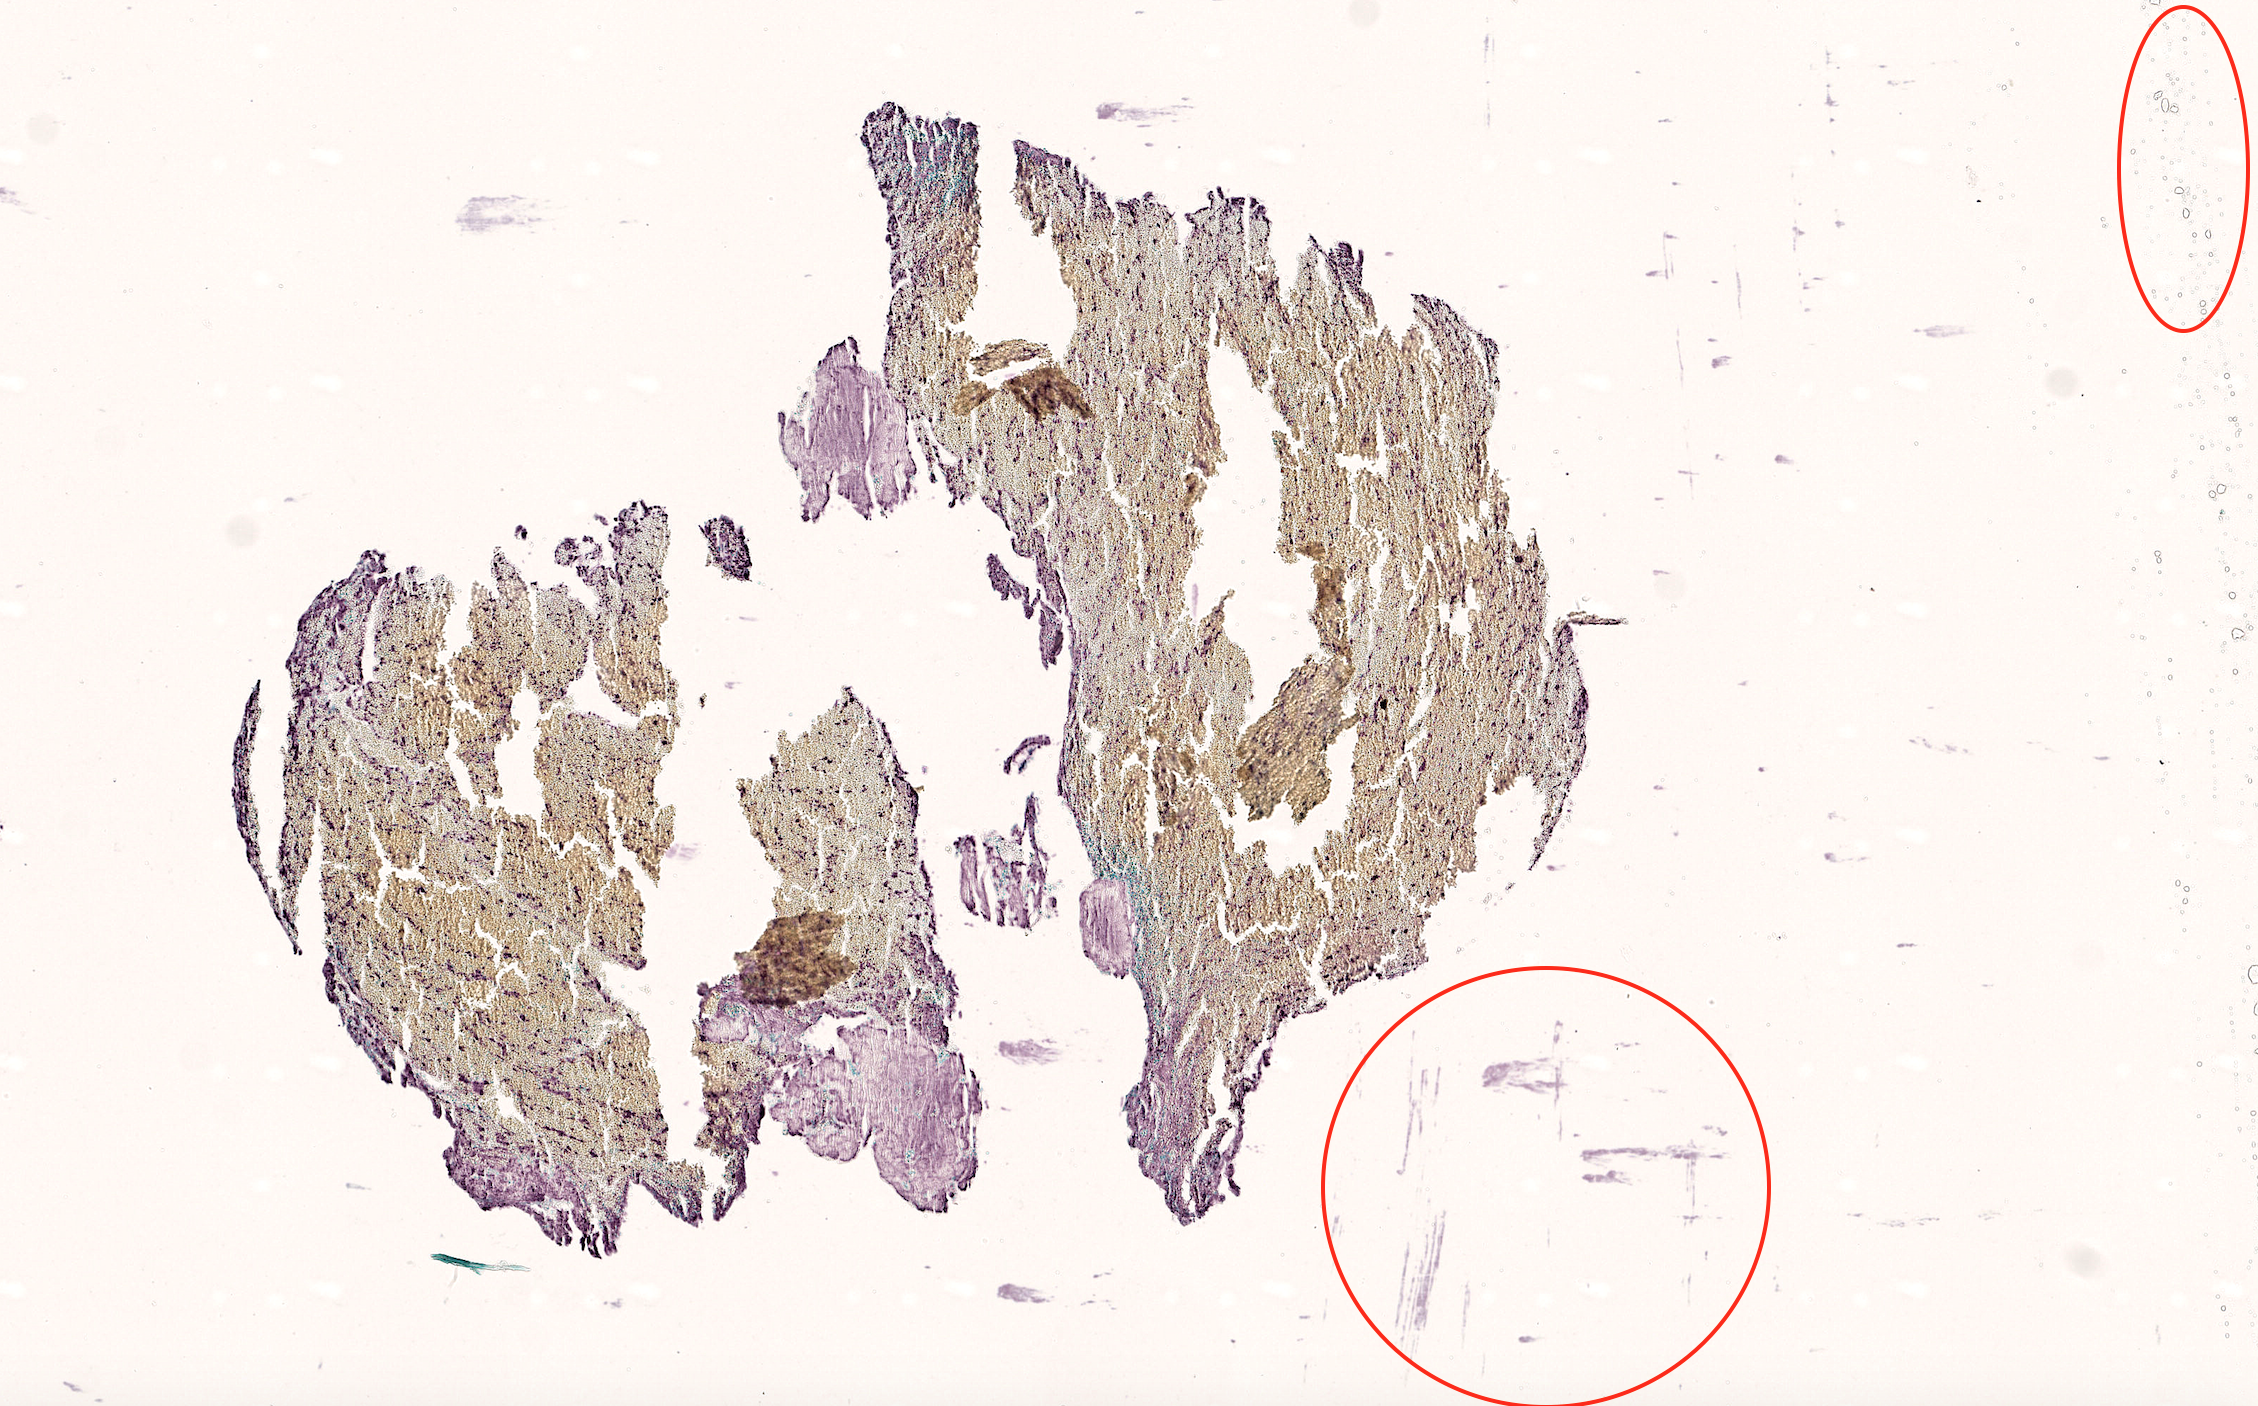
\includegraphics[width = \textwidth]{Ruis_afbeelding.png}
	
	\caption{In de rechterbovencirkel zien we luchtbellen en in de onderste cirkel zien we een verkleuring die geen deel uitmaakt van de bloedklonter.}
	\label{figuur 1}
\end{figure}

\subsection{Lokalisatie van de indicator}
Het tweede en ietwat moeilijkere deel is om uiteindelijk de indicators te lokaliseren. Hier zullen we twee soorten onderscheiden. Een voorbeeld is te zien op de volgende figuren \ref{figuur 2}. Het kleurverschil tussen indicator en achtergrond is niet al te groot waardoor we het oorspronkelijke \textit{RGB} kleurmodel \footnote{Het RGB kleurmodel is een voorstelling waarbij ieder kleur voorgesteld wordt door een waarde van de drie basiskleuren(rood, groen en blauw)} omvormen naar het zogenaamde \textit{HSV} kleurmodel. Dit model is een alternatieve voorstelling waarbij men alle kleuren op een cirkel voorstelt, de hoek die dit kleur maakt, noemt men de \textit{Hue}. Naast deze waarde heeft \textit{HSV} nog twee andere parameters namelijk \textit{Saturation} en \textit{Value}. \textit{Saturation} kan simpel beschouwd worden als een aanduiding van de hoeveelheid witte kleur en \textit{Value} een aanduiding van de zwarte kleur. Een grafisch overzicht is te zien op figuur \ref{figuur 3}
\begin{figure}[H]
	\centering
	\subfloat[]{{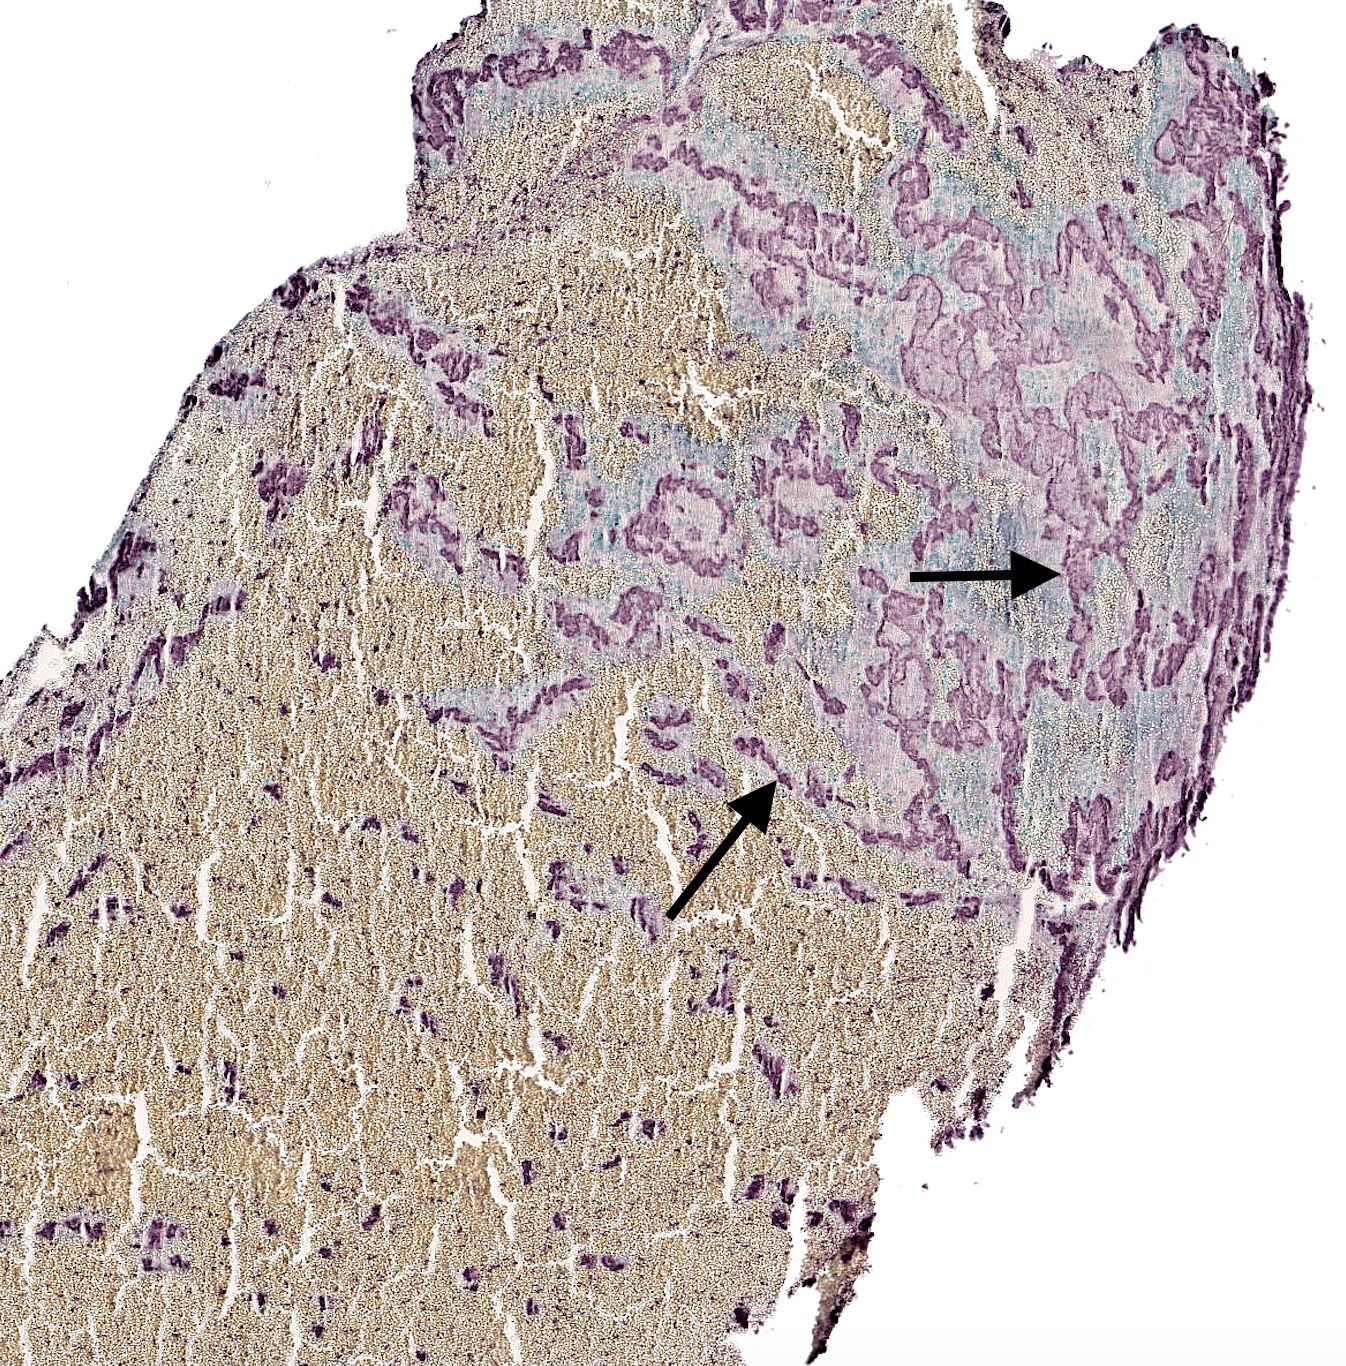
\includegraphics[width=7.5cm]{Indicator_vb1}}}
	\qquad
	\subfloat[]{{\includegraphics[width=7.5cm]{Indicator_vb2}}}
	
	\caption{Illustratie van de twee soorten indicator (respectievelijk paars en donkerroze) die gedetecteerd moeten worden. We zien duidelijk dat het detecteren op afbeelding (a) eenvoudiger zal zijn dan op afbeelding (b)}
	\label{figuur 2}
\end{figure}
\begin{figure}[H]
	\centering
	\includegraphics[]{HSV_vb.png}
	
	\caption{Grafische voorstelling van het HSV kleurmodel}
	\label{figuur 3}
\end{figure}
Het voordeel van deze transformatie is dat het heel wat eenvoudiger is om een onderscheid tussen dichtbijgelegen kleuren te vinden. Een andere mogelijke transformatie is die naar het \textit{Lab} kleurmodel die nog een alternatieve representatie en mogelijke optie is.\\
Bij het bestuderen van de \textit{HSV} waarden is er hopelijk een onderscheid tussen de indicatoren en de rest van de bloedklonter te zien. Eens dit onderscheid experimenteel te bepalen is, kunnen we een statistische analyse van de data doen. Het is namelijk de bedoeling dat we op iedere foto en niet op slechts één foto een goed onderscheid kunnen maken. Dit doen we door eerst alle pixels die met zekerheid een indicator zijn te detecteren en deze dan onderling te verbinden. \\
Wanneer we eenmaal alle pixels gevonden hebben, is het niet moeilijk om het percentage van de indicator op de bloedklonter te berekenen. Dit is niet veel meer dan de verhouding \(indicatorpixels/bloedklonterpixels\).

\section*{Besluit}

Afsluitende tekst

\end{document}
